%-----------------------------------------------------------------------------%
\chapter{\babTiga}
%-----------------------------------------------------------------------------%
Metode yang digunakan dalam penelitian ini adalah metode kuantitatif dengan melakukan pengukuran akurasi dari pengujian data tes terhadap model yang terbentuk.


%-----------------------------------------------------------------------------%
\section{Teknik Pengumpulan Data}
%-----------------------------------------------------------------------------%
Sebelum melakukan penelitian, terlebih dahulu dilakukan proses pengumpulan data. Teknik yang digunakan untuk melakukan pengumpulan data adalah sebagai berikut:
\begin{enumerate}
	\item Studi literatur.\\
Sebelum mengumpulkan data, dilakukan proses studi literatur untuk menemukan jenis data yang tepat untuk melakukan penelitian ini.	
	\item Pengambilan data.\\
Proses pengambilan data dilakukan dengan mencari menggunakan teknologi internet dan search engine, misalnya dengan keyword “batik”, “batik Indonesia”, dll. Selain itu, dilakukan pengumpulan data secara langsung ke museum tekstil di Jakarta.
\end{enumerate}

%-----------------------------------------------------------------------------%
\section{Data}
Data yang digunakan dalam penelitian ini merupakan data primer yang diambil berdasarkan kata kunci di internet maupun pengambilan secara langsung seperti yang telah dijelaskan pada butir 3.1. Dalam penelitian ini, terdapat dua jenis data, yaitu data latih dan data uji. \\
Data latih yang diperlukan adalah kumpulan data batik yang memiliki variasi motif yang berasal dari berbagai daerah di Indonesia.

\section{Rancangan Penelitian}
Penelitian ini dilakukan di Fasilkom UI dengan metode penelitian kuantitatif yaitu dengan mengukur ketepatan prediksi asal daerah batik dari motif kain. Metode yang digunakan untuk membuat model prediksi motif kain adalah CNN dimana input akan dipecah menjadi ukuran yang lebih kecil dan diproses kedalam beberapa layer sehingga akan ditemukan fitur dari gambar yang kemudian menghasilkan model untuk melakukan deteksi asal daerah batik dari pola kain.\\
Alur kegiatan yang dilakukan dalam penelitian ini terdiri dari langkah, yaitu identifikasi masalah, studi literatur, pengumpulan data, Implementasi CNN, Implementasi Web Service, Implmentasi Web Service Client, Latih CNN, Uji CNN, Analisis hasil, Penarikan kesimpulan dan pembuatan laporan. Langkah-langkah tersebut dapat digambarkan dalam alur proses yang dapat dilihat pada gambar 3.1. Adapun target durasi waktu kerja dari langkah-langkah pada alur yang digambarkan pada tabel 3.2 dapat dilihat pada table project plan sebagai berikut.\\
\begin{table}
	\centering
	\caption{Project plan penelitian pengenalan batik dengan android}
	\label{tab:tab1}
	\begin{tabular}{| l|l|}
		\hline
		No & Deskripsi \\ 
		\hline
		1 & Identifikasi Masalah \\
		\hline
		2 & Studi Literatur \\
		\hline
		3 & Pengumpulan Data \\
		\hline
		4 & Implementasi CNN\\
		\hline
		5 & Implementasi Web Service\\				
		\hline
		6 & Implementasi Web Service Client\\
		\hline
		7 & Pelatihan CNN\\
		\hline
		8 & Pengujian CNN\\
		\hline
		9 & Analisis Hasil \\
		\hline
		10 & Penarikan Kesimpulan\\
		\hline
		11 & Pembuatan Laporan\\
		\hline
	\end{tabular}
\end{table}
\begin{table}
	\centering
	\caption{Timeline penelitian pengenalan batik dengan android}
	\label{tab:tab1}
	\begin{tabular}{|l|l|l|l|l|l|l|l|}
		\hline
		No & Deskripsi & Jul & Aug & Sep & Oct & Nov & Dec\\ 
		\hline
		1 & Identifikasi Masalah &x&&&&&\\
		\hline
		2 & Studi Literatur&x&&&&&\\
		\hline
		3 & Pengumpulan Data&&x&&&&\\
		\hline
		4 & Implementasi CNN&&x&x&x&&\\
		\hline
		5 & Implementasi Web Service&&x&x&x&&\\
		\hline
		6 & Implementasi Web Service Client&&x&x&x&&\\
		\hline
		7 & Pelatihan CNN&&x&x&x&&\\
		\hline
		8 & Pengujian CNN&&x&x&x&&\\
		\hline
		9 & Analisis Hasil&&&&&x&\\
		\hline
		10 & Penarikan Kesimpulan&&&&&x&\\
		\hline
		11 & Pembuatan Laporan&&&&&&x\\
		\hline
	\end{tabular}
\end{table}
Pengambilan data dilakukan pada bulan Maret 2016 pada museum tekstil jakarta, sedangkan pengambilan data via internet, dilakukan dari awal januari 2016 hingga saat ini.

\section{Pelatihan Model CNN}
Pelatihan motif kain dimulai dari input gambar yang sudah diberikan label secara manual berdasarkan kata kunci pencarian pada internet berdasarkan daerah asal batik dan data yang disediakan oleh museum tekstil. Gambar akan dijadikan input pada deeplearning4j dengan inisialisasi parameter:
\begin{itemize}
\item Seed
\item Iterations
\item Regularizations
\item L2
\item Learning rate
\item Weightinit
\item Optimization Algorithm
\item Updater
\end{itemize}

Setelah melakukan inisialisasi parameter, data gambar akan diproses kedalam layer dengan urutan sbb:
\begin{itemize}
	\item Layer 0 : Convolution Layer
	\item Layer 1 : Subsampling Layer  Max Pooling
	\item Layer 2 : Convolution Layer
	\item Layer 3 : Subsampling Layer  Max Pooling
	\item Layer 4 : Dense Layer
	\item Layer 5 : Output Layer
\end{itemize}

\begin{figure}[htp]
	\centering
	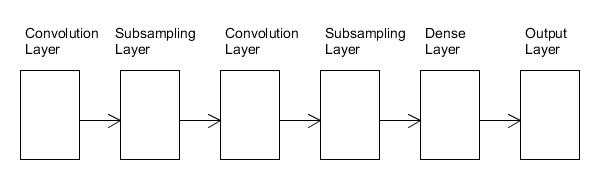
\includegraphics[width=8cm]{pics/arsitektur_cnn}
	\caption{Arsitektur CNN}
	\label{fig:arsitektur_cnn}
\end{figure}
Hasil dari output layer akan melakukan evaluasi terhadap data testing dan dilakukan pengukuran nilai . model hasil pembelajaran deeplearning4j akan disimpan dalam bentuk file biner sehingga bisa digunakan kembali untuk melakukan deteksi daerah asal kain batik.
\begin{figure}[htp]
	\centering
	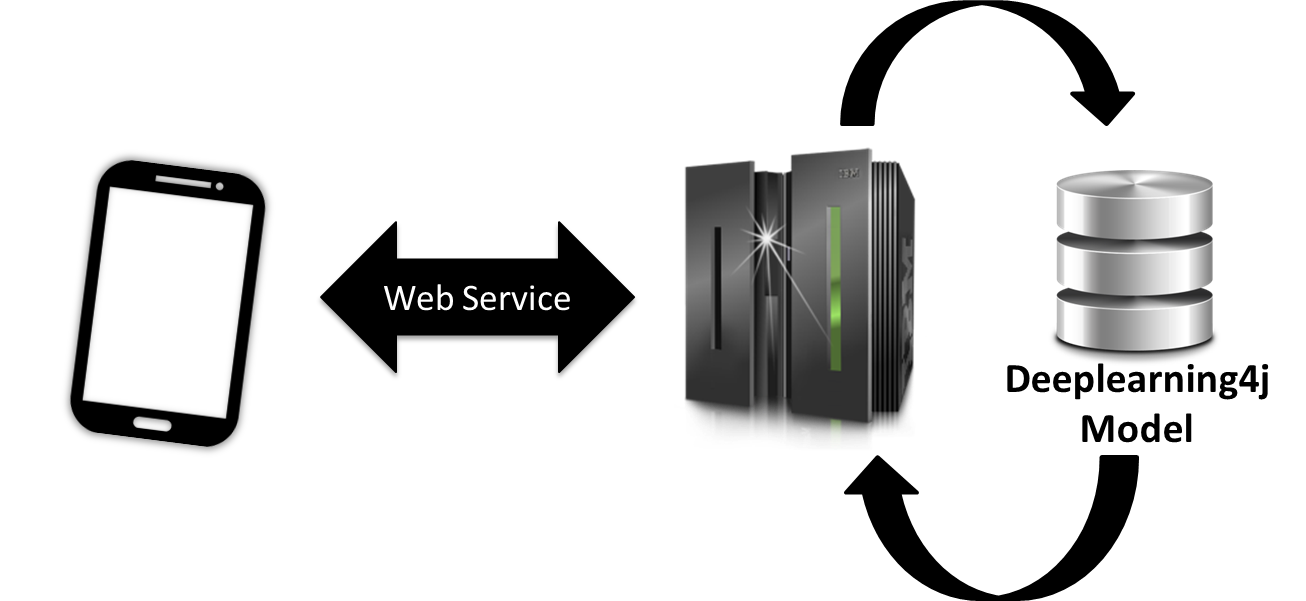
\includegraphics[width=8cm]{pics/komunikasi_cnn}
	\caption{Arsitektur Server untuk CNN}
	\label{fig:komunikasi_cnn}
\end{figure}